\subsection{$d(K^-, p)"\pi^-\Sigma^0"$ and $d(K^-, p)"\pi^-\Lambda"$ cross section}
\begin{figure}[htbp]
  \centering
  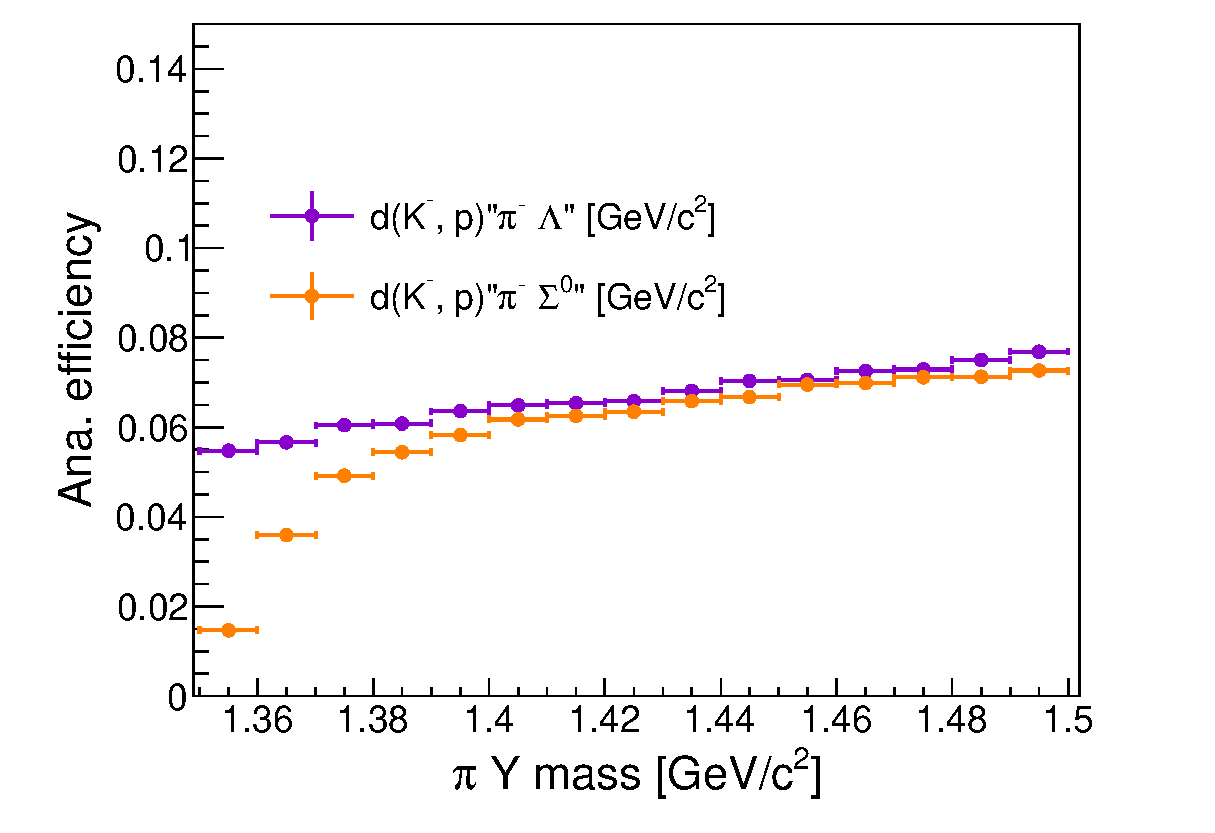
\includegraphics[width=8cm]{../pic/Run68/KP_ana/kp_acc.eps}
  \caption{
    This figure shows acceptanes of the $d(K^-, p)"\pi^-Sigma^0$ and the $d(K^-, p)"\pi^-\Lambda"$ which was estimated by the Monte Calro simulation.
  }
  \label{fig:acc_kp}
\end{figure}

The $d(K^-, p)"\pi^-\Sigma^0"$ and the $d(K^-, p)"\pi^-\Lambda"$ spectra was converted to the corss section to collected accpetance.
For this, we performed the Monte Carlo simulation using geant4 toolkit which was described in detail in Sec\ref{sec:geant4}.
In this simulation, proton was generated at forward angle which is within $\theta<8$ degree.
Since this simulation's purpose was evaluation of the CDS acceptance, we used proton pass through PC/CVC as denominator events.
We estimated effective events to adopt same analysis procedure to Monte Carlo simulations data,
so the efficeincy incudes analysis efficiency which is PID selection of the CDS and each gete for particles and so on.
For the acceptance estimation of these reactions, we simulated  $K^- d\rightarrow \pi^- \Sigma^0 p_{forward}$  and $K^- d \rightarrow \pi^- \Lambda p_{forward}$ reactions.
In this simulation, masses of $\pi^-\Sigma^0$/$\pi^-\Lambda$ were adopted flat distribution for same statistics in region of interest.

We obtain corss sections of the $d(K^-, p)"\pi-\Sigma^0"$ and the $d(K^-, p)"\pi^-\Lambda$ to be corrected by acceptance.
Fig\ref{fig:pimS0_CS}-\ref{fig:pimL_CS} show obtained coross sections.
In these figures, statical errors which is dependent error for each bins was indicated using boxes and
errors which was convolved error of conversion factor parameters that is common in all bins was indicated as error bars.

\begin{figure}[htbp]
  \centering
  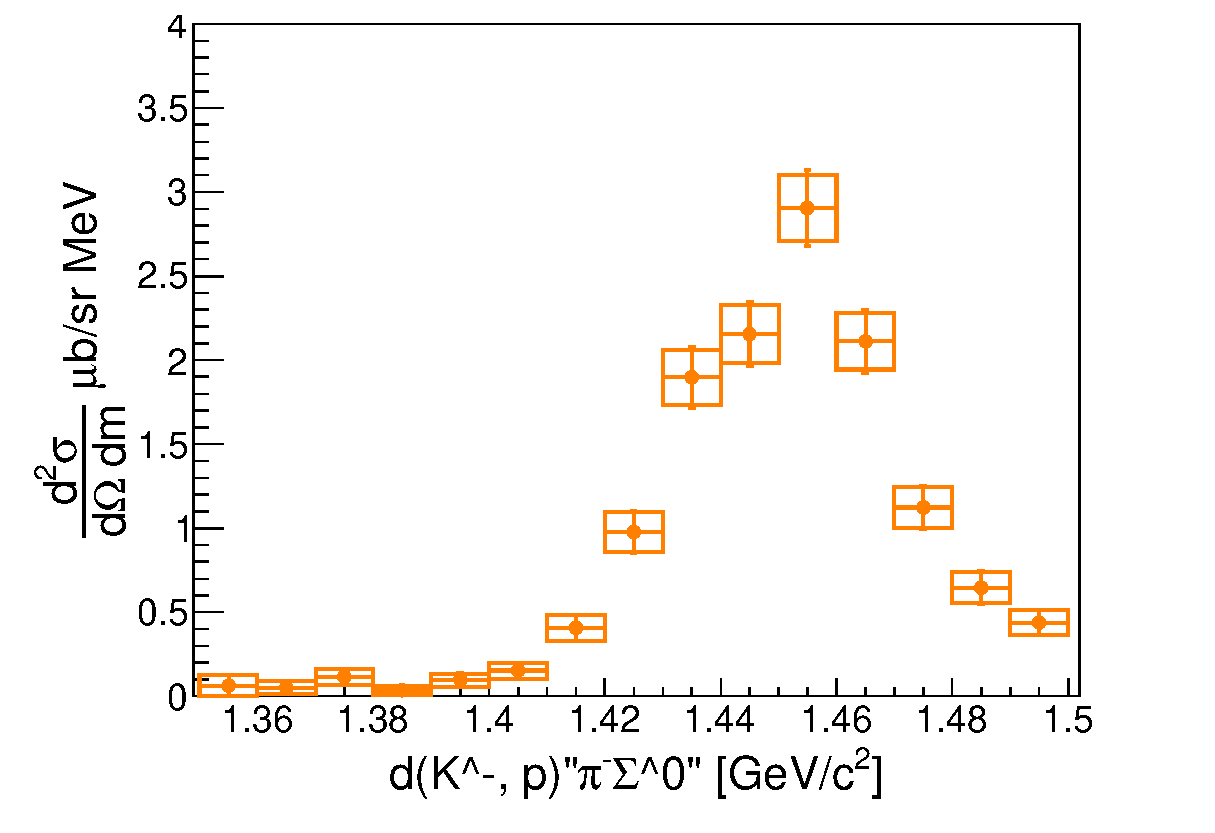
\includegraphics[width=10cm]{../pic/Run68/KP_ana/pimS0_CS_zoom.eps}
  \caption{
    The cross section of $d(K^-, p)"\pi^-\Sigma^0$ mode.
  }
  \label{fig:pimS0_CS}
\end{figure}

\begin{figure}[htbp]
  \centering
  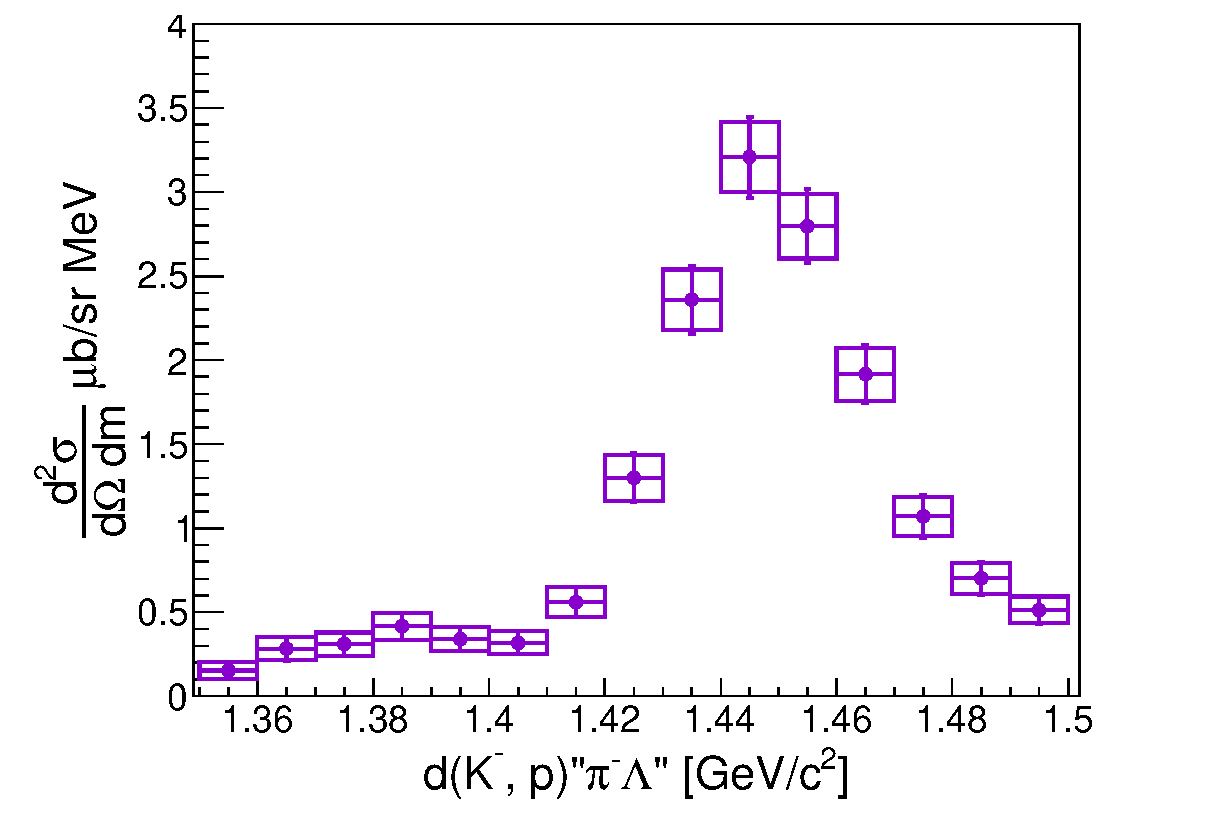
\includegraphics[width=10cm]{../pic/Run68/KP_ana/pimL_CS_zoom.eps}
  \caption{
    The cross section of $d(K^-, p)"\pi^-\Lambda^0$ mode.
  }
  \label{fig:pimL_CS}
\end{figure}

